\documentclass[water,article,submit,pdftex,moreauthors]{Definitions/mdpi}
%DIF LATEXDIFF DIFFERENCE FILE
%DIF DEL main-old.tex   Thu Jul  4 23:07:36 2024
%DIF ADD main.tex       Thu Jul  4 23:07:24 2024

% %%
% document
%DIF PREAMBLE EXTENSION ADDED BY LATEXDIFF
%DIF UNDERLINE PREAMBLE %DIF PREAMBLE
\RequirePackage[normalem]{ulem} %DIF PREAMBLE
\RequirePackage{color}\definecolor{RED}{rgb}{1,0,0}\definecolor{BLUE}{rgb}{0,0,1} %DIF PREAMBLE
\providecommand{\DIFadd}[1]{{\protect\color{blue}\uwave{#1}}} %DIF PREAMBLE
\providecommand{\DIFdel}[1]{{\protect\color{red}\sout{#1}}}                      %DIF PREAMBLE
%DIF SAFE PREAMBLE %DIF PREAMBLE
\providecommand{\DIFaddbegin}{} %DIF PREAMBLE
\providecommand{\DIFaddend}{} %DIF PREAMBLE
\providecommand{\DIFdelbegin}{} %DIF PREAMBLE
\providecommand{\DIFdelend}{} %DIF PREAMBLE
\providecommand{\DIFmodbegin}{} %DIF PREAMBLE
\providecommand{\DIFmodend}{} %DIF PREAMBLE
%DIF FLOATSAFE PREAMBLE %DIF PREAMBLE
\providecommand{\DIFaddFL}[1]{\DIFadd{#1}} %DIF PREAMBLE
\providecommand{\DIFdelFL}[1]{\DIFdel{#1}} %DIF PREAMBLE
\providecommand{\DIFaddbeginFL}{} %DIF PREAMBLE
\providecommand{\DIFaddendFL}{} %DIF PREAMBLE
\providecommand{\DIFdelbeginFL}{} %DIF PREAMBLE
\providecommand{\DIFdelendFL}{} %DIF PREAMBLE
%DIF COLORLISTINGS PREAMBLE %DIF PREAMBLE
\RequirePackage{listings} %DIF PREAMBLE
\RequirePackage{color} %DIF PREAMBLE
\lstdefinelanguage{DIFcode}{ %DIF PREAMBLE
%DIF DIFCODE_UNDERLINE %DIF PREAMBLE
  moredelim=[il][\color{red}\sout]{\%DIF\ <\ }, %DIF PREAMBLE
  moredelim=[il][\color{blue}\uwave]{\%DIF\ >\ } %DIF PREAMBLE
} %DIF PREAMBLE
\lstdefinestyle{DIFverbatimstyle}{ %DIF PREAMBLE
	language=DIFcode, %DIF PREAMBLE
	basicstyle=\ttfamily, %DIF PREAMBLE
	columns=fullflexible, %DIF PREAMBLE
	keepspaces=true %DIF PREAMBLE
} %DIF PREAMBLE
\lstnewenvironment{DIFverbatim}{\lstset{style=DIFverbatimstyle}}{} %DIF PREAMBLE
\lstnewenvironment{DIFverbatim*}{\lstset{style=DIFverbatimstyle,showspaces=true}}{} %DIF PREAMBLE
%DIF END PREAMBLE EXTENSION ADDED BY LATEXDIFF

\usepackage{algorithm}
\usepackage{algorithmic}

% MDPI internal commands - do not modify
\firstpage{1}
\makeatletter
\setcounter{page}{\@firstpage}
\makeatother
\pubvolume{1}
\issuenum{1}
\articlenumber{0}
\pubyear{2024}
\copyrightyear{2024}
%\externaleditor{Academic Editor: Firstname Lastname}
\datereceived{ }
\daterevised{ } % Comment out if no revised date
\dateaccepted{ }
\datepublished{ }
%\datecorrected{} % For corrected papers: "Corrected: XXX" date in the original paper.
%\dateretracted{} % For corrected papers: "Retracted: XXX" date in the original paper.
\hreflink{https://doi.org/} % If needed use \linebreak
%\doinum{}
%\pdfoutput=1 % Uncommented for upload to arXiv.org
%\CorrStatement{yes}  % For updates


% %% preamble
% Full title of the paper (Capitalized)
\Title{A Stream Order Family and Order-Based Parallel River Network Routing Method}

% MDPI internal command: Title for citation in the left column
\TitleCitation{A stream order family and order based parallel river network routing method}

% Author Orchid ID: enter ID or remove command
\newcommand{\orcidauthorZ}{0000-0001-7580-9128}

% Authors, for the paper (add full first names)
\Author{Xi Yang $^{1}$, Chong Wei $^{1}$, Zhiping Li $^{2}$, Heng Yang $^{3}$ and Hui Zheng $^{4,}$*\orcidZ{}}

% MDPI internal command: Authors, for metadata in PDF
\AuthorNames{Xi Yang, Chong Wei, Zhiping Li, Heng Yang, and Hui Zheng}

% MDPI internal command: Authors, for citation in the left column
\AuthorCitation{Yang, X.; Wei, C.; Li, Z.; Yang, H.; Zheng, H.}

% Affiliations / Addresses (Add [1] after \address if there is only one affiliation.)
\address{%
$^{1}$ \quad College of Surveying and Geo-Informatics, North China University of Water Resources and Electric Power, Zhengzhou 450046, China; yangxi940822@gmail.com (X.Y.); dixin313@163.com (C.W.)\\
$^{2}$ \quad College of Geosciences and Engineering, North China University of Water Resources and Electric Power, Zhengzhou 450045, China; lizhiping@ncwu.edu.cn (Z.L.)\\
$^{3}$ \quad Science and Technology Research Institute, China Three Gorges Corporation, Beijing 100038, China; yang\_heng2@ctg.com.cn (H.Y.)\\
$^{4}$ \quad Laboratory of Regional Climate-Environment Research for Temperate East Asia, Institute of Atmospheric Physics, Chinese Academy of Sciences, Beijing 100029, China; zhenghui@tea.ac.cn (H.Z.) }

% Contact information of the corresponding author
\corres{Correspondence: zhenghui@tea.ac.cn}

% Abstract (Do not insert blank lines, i.e. \\)
%DIF 59c59
%DIF < \abstract{River network routing is fundamental for flood forecasting but becomes computationally demanding with networks comprising thousands to millions of reaches. The sequential nature of upstream-to-downstream flow paths within river networks poses a significant challenge for parallel computation. This study introduces a family of stream orders coupled with an order-based parallel routing approach. We assign each reach an order that falls between one more than the maximum order of its upstream reaches and one less than the order of its downstream reach. This strategy enables parallel simulation of reaches with identical orders while sequentially processing those with different orders, thus maintaining the crucial upstream-to-downstream dynamic. To further enhance parallel scalability, we strategically relax the upstream-to-downstream relationship along the longest flow paths, dividing the network into independent subnetworks and introducing halo reaches to mitigate the impact of inexact inflows. We validate our approach using China's Yangtze River basin, the country's largest river network with 53,600 fully connected reaches. Employing a conceptual parallel execution machine, we demonstrate that our method achieves 80\% parallel efficiency with up to 25 processors. By strategically introducing breakpoints, we further enhance scalability, enabling efficient simulations on 77 processors while maintaining 80\% efficiency. These results highlight the scalability and efficiency of our methods for large-scale, high-resolution river network modeling within Earth system models. Our study also lays a theoretical groundwork for optimizing stream orders and halo reach placements, crucial for advancing river network modeling.}
%DIF -------
\abstract{\DIFdelbegin \DIFdel{River network routing is fundamental for flood forecasting but becomes computationally demanding with networks comprising thousands to millions of reaches. T}\DIFdelend \DIFaddbegin \DIFadd{River network routing's significance in reach-level flood forecasting over extensive domains is growing, requiring considerable computational resources for modeling networks comprising thousands to millions of reaches. Parallel computation plays a central role in timely forecasting in such cases. However, t}\DIFaddend he sequential nature of upstream-to-downstream flow paths within river networks poses a significant challenge for parallelization. This study introduces a family of stream orders coupled with an order-based parallel routing approach. We assign each reach an order that falls between one more than the maximum order of its upstream reaches and one less than the order of its downstream reach. This strategy enables the parallel simulation of reaches with identical orders while sequentially processing those with different orders, thus maintaining the crucial upstream-to-downstream dynamic. To further enhance parallel scalability, we strategically relax the upstream-to-downstream relationship along the longest flow paths, dividing the network into independent subnetworks and introducing halo reaches to mitigate the impact of inexact inflows. We validate our approach using China's Yangtze River basin, the country's largest river network with 53,600 fully connected reaches. Employing a conceptual parallel execution machine, we demonstrate that our method achieves 80\% parallel efficiency with up to 25 processors. By strategically introducing breakpoints, we further enhance scalability, enabling efficient simulations on 77 processors while maintaining 80\% efficiency. These results highlight the scalability and efficiency of our methods for large-scale, high-resolution river network modeling within Earth system models. Our study also lays a theoretical groundwork for optimizing stream orders and halo reach placements, crucial for advancing river network modeling.} %DIF >
%DIF -------

% Keywords
\keyword{stream order; river network routing; parallel computing; flood}

\begin{document}

\section{Introduction}

River \DIFdelbegin \DIFdel{networks play an essential role in the terrestrial water cycle~\mbox{%DIFAUXCMD
        \cite{trenberth2007JHM}}\hskip0pt%DIFAUXCMD
    . They serve as the primary conveyance systems for water, linking terrestrial and aquatic ecosystems, and facilitating the transport of water, sediment, nutrients, and pollutants across diverse landscapes~\mbox{%DIFAUXCMD
        \cite{dai2002JHM, dai2009JC, regnier2022N, sohail2022N, liu2019NC, li2019JAMES, aufdenkampe2011FEE}}\hskip0pt%DIFAUXCMD
    . The representation of river network routing is a critical component in the development and refinement of land surface models and Earth system models~\mbox{%DIFAUXCMD
        \cite{david2016ESS}}\hskip0pt%DIFAUXCMD
    . The fidelity with which land surface models or Earth system models capture the spatial and temporal dynamics of river networks directly influences the models' ability to simulate key hydrological processes, such as evapotranspiration, infiltration, and runoff~\mbox{%DIFAUXCMD
        \cite{senatore2015JAMES, wagner2016WRR}}\hskip0pt%DIFAUXCMD
    . Moreover, }\DIFdelend \DIFaddbegin \DIFadd{network routing has become increasingly essential for flood forecasting at the reach level over large domains, such as entire nations or even globally, as demonstrated by various studies~\mbox{%DIFAUXCMD
        \cite{alfieri2013HESS, david2016ESS, maidment2017JAWRA, lin2018JHM, read2023JAWRA}}\hskip0pt%DIFAUXCMD
    . The National Water Model of }\DIFaddend the \DIFdelbegin \DIFdel{routing of water through river networks is a critical control on the timing and magnitude of floods~\mbox{%DIFAUXCMD
        \cite{lin2018JHM, alfieri2013HESS}}\hskip0pt%DIFAUXCMD
    .
    As such, the inclusion of the detailed, fine-scale river network routing is not only vital for improving our understanding of the terrestrial water cycle but also for informing flood defense in regions where flood risk is a pressing concern~\mbox{%DIFAUXCMD
        \cite{willner2018NCC}}\hskip0pt%DIFAUXCMD
    . }\DIFdelend \DIFaddbegin \DIFadd{United States stands out as a successful example. It has been operational since 2016, providing flood forecasts for millions of reaches across the country. Its forecasts have effectively guided emergency responses during Hurricane Harvey~\mbox{%DIFAUXCMD
        \cite{maidment2017JAWRA, read2023JAWRA}}\hskip0pt%DIFAUXCMD
    . The Global Flood Awareness System is another significant example. Its forecasts cover the entire globe, including data-scarce regions. The forecasts have demonstrated their value for targeted humanitarian disaster prevention actions in countries such as Uganda~\mbox{%DIFAUXCMD
        \cite{alfieri2013HESS, coughlan_de_perez2016HESS}}\hskip0pt%DIFAUXCMD
    . More large-domain flood forecasting systems that leverage river network routing are actively being developed worldwide, including the recently established European-wide Flood Early Warning System~\mbox{%DIFAUXCMD
        \cite{najafi2024NC, thober2019GMD}}\hskip0pt%DIFAUXCMD
    .
}\DIFaddend

\DIFdelbegin \DIFdel{Land surface models and Earth system models strive to capture the intricate details of river networks~\mbox{%DIFAUXCMD
        \cite{lehner2013HP, yamazaki2019WRR, chaney2021GMD} }\hskip0pt%DIFAUXCMD
    over large domains, such as entire nations or the globe~\mbox{%DIFAUXCMD
        \cite{yang2021BAMS, lin2019WRR, wu2012WRR, alfieri2013HESS}}\hskip0pt%DIFAUXCMD
    . Fine-scale river network routing, which requires short river reaches and }\DIFdelend \DIFaddbegin \DIFadd{River network routing in flood forecasts is urgently focusing on shorter reaches~\mbox{%DIFAUXCMD
        \cite{maidment2017JAWRA, coughlan_de_perez2016HESS, najafi2024NC, wada2016JAMES}}\hskip0pt%DIFAUXCMD
    . The use of shorter reaches and the accompanying }\DIFaddend frequent time-stepping \DIFdelbegin \DIFdel{, }\DIFdelend is crucial for \DIFdelbegin \DIFdel{accurately simulating water flow through the complex channels of a river network. This level of detail is crucial for resolving small-scale }\DIFdelend \DIFaddbegin \DIFadd{resolving fine-scale }\DIFaddend features and processes that \DIFdelbegin \DIFdel{can }\DIFdelend significantly impact larger-scale river water flow patterns~\cite{yamazaki2009HESS, thober2019GMD, mizukami2021JAMES, nguyen-quang2018GMD}\DIFaddbegin \DIFadd{. This resolution of fine-scale water flow features within the river network enables local flood impact assessments to be highly relevant to individual people and infrastructures. These assessments are essential, providing targeted information instrumental for effective disaster prevention and response actions~\mbox{%DIFAUXCMD
        \cite{maidment2017JAWRA, coughlan_de_perez2016HESS}}\hskip0pt%DIFAUXCMD
    .
}

\DIFadd{Large-domain }\DIFaddend and \DIFdelbegin \DIFdel{is essentialfor action-based flood forecasting~\mbox{%DIFAUXCMD
        \cite{wada2016JAMES, coughlan_de_perez2016HESS}}\hskip0pt%DIFAUXCMD
    .
    The computational demand associated with the }\DIFdelend fine-scale river network routing \DIFdelbegin \DIFdel{over a large domain is substantial }\DIFdelend \DIFaddbegin \DIFadd{demands substantial computational resources}\DIFaddend ~\cite{yamazaki2013WRR, liu2014EMS, mizukami2021JAMES, david2015WRR, liu2023JH}. \DIFdelbegin \DIFdel{Moreover, the integration of fine-scale river routing with other model components, such as nutrient transport and human water use ~\mbox{%DIFAUXCMD
        \cite{wada2016JAMES}}\hskip0pt%DIFAUXCMD
    , further compounds the computational load. As a result, researchers and model developers }\DIFdelend \DIFaddbegin \DIFadd{Considering the constraints imposed by limited computational resources, flood forecasting systems }\DIFaddend must balance the \DIFdelbegin \DIFdel{desire for high-fidelity river network representation with the practical constraints of computational feasibility. The ongoing advancements in high-performance computing and the development of more sophisticated numerical methods are key to addressing these computational challenges~\mbox{%DIFAUXCMD
        \cite{yamazaki2013WRR, liu2014EMS, mizukami2021JAMES, david2015WRR, liu2023JH} }\hskip0pt%DIFAUXCMD
    and enabling the next generation of Earth system models and land surface models to incorporate large-domain }\DIFdelend \DIFaddbegin \DIFadd{need for detailed }\DIFaddend fine-scale \DIFdelbegin \DIFdel{river network routing effectively.
}%DIFDELCMD <

%DIFDELCMD < %%%
\DIFdel{The }\DIFdelend \DIFaddbegin \DIFadd{modeling over broad domains with the necessity of timely forecasts. To reconcile these competing demands, the }\DIFaddend implementation of parallel processing in river network routing is essential\DIFdelbegin \DIFdel{for enhancing }\DIFdelend \DIFaddbegin \DIFadd{. Parallel processing is crucial for enhancing computational efficiency and directly contributes to meeting the timeliness requirements of flood forecasts.
}

\DIFadd{However, }\DIFaddend the \DIFdelbegin \DIFdel{performance of large-domain fine-scale simulations.
    However, this approach introduces considerable challenges. A primary concern stems from the inherently distributed structure of river networks, where numerous tributaries and river segments are intricately interconnected. This necessitates advanced data management protocols and parallel computation strategies to facilitate accurate information exchange regarding water flow dynamics between different segments of the river network~\mbox{%DIFAUXCMD
        \cite{liu2023JH}}\hskip0pt%DIFAUXCMD
    . It is imperative that this information exchange preserves the integrity of the upstream-to-downstream flow sequence, as the }\DIFdelend \DIFaddbegin \DIFadd{parallelization of river network routing presents considerable challenges, primarily due to the inherent sequential nature of the river flow from upstream to downstream within the networks. The }\DIFaddend flow in any given \DIFdelbegin \DIFdel{segment is contingent upon }\DIFdelend \DIFaddbegin \DIFadd{reach is dependent on }\DIFaddend the flow conditions in its upstream \DIFdelbegin \DIFdel{segments. Parallelization must respect this sequential dependencyto ensure that the simulation outcomes are physically plausible and precise~\mbox{%DIFAUXCMD
        \cite{david2013WRR, mizukami2021JAMES, liu2014EMS, liu2023JH}}\hskip0pt%DIFAUXCMD
    . }%DIFDELCMD <

%DIFDELCMD < %%%
\DIFdel{The inherent sequential nature of river flow significantly impedes the development of efficient and scalable parallel processing methods for river network routing }\DIFdelend \DIFaddbegin \DIFadd{reaches. It is imperative that a parallel routing algorithm respects this upstream-to-downstream dependency}\DIFaddend . \DIFdelbegin \DIFdel{Furthermore}\DIFdelend \DIFaddbegin \DIFadd{When this dependency is a constraint, the parallel routing needs to revert to a sequential approach from upstream to downstream. Additionally}\DIFaddend , the spatial variability within river networks, marked by differences in channel widths, slopes, and flow velocities, adds to the complexity of parallelization. This variability necessitates dynamic load balancing techniques to prevent computational resources from being underutilized or overburdened. \DIFdelbegin \DIFdel{The development of robust parallel schemes is therefore critical to }\DIFdelend \DIFaddbegin \DIFadd{Consequently, it is critical to develop robust parallel algorithms that can }\DIFaddend accommodate the diverse \DIFdelbegin \DIFdel{scales and dynamics inherent to river networks , without compromising the fidelity or reliability of the model's projections}\DIFdelend \DIFaddbegin \DIFadd{dynamics and inherent sequentiality within river networks effectively, ensuring that simulation results are physically plausible and accurate~\mbox{%DIFAUXCMD
        \cite{david2013WRR, mizukami2021JAMES, liu2014EMS, liu2023JH}}\hskip0pt%DIFAUXCMD
}\DIFaddend .

\DIFdelbegin \DIFdel{Various methods existfor parallelizing river network routing}\DIFdelend \DIFaddbegin \DIFadd{Several parallelization methods exist}\DIFaddend , such as domain decomposition~\cite{mizukami2021JAMES, liu2023JH} and halo reaches~\cite{david2013WRR}. Domain decomposition involves partitioning river networks into independent tributaries and interconnected mainstreams. The tributaries are then allocated to various processors for concurrent simulation, while the mainstreams are processed in an upstream-to-downstream sequence. However, the parallelization scalability is limited. As the number of processors increases, the distribution of reaches within the tributaries diminishes, and the mainstream reaches become more dominant~\cite{mizukami2021JAMES}. In an extreme scenario with an infinite number of processors, the majority of river reaches would be classified as mainstreams, effectively rendering the routing process predominantly sequential.

With the halo-reach method, the river network is divided into independent subnetworks, each of which is simulated in parallel without maintaining an upstream-to-downstream relationship at their boundaries~\cite{david2015WRR}. To mitigate the inaccuracies arising from this \DIFaddbegin \DIFadd{artificial }\DIFaddend division, halo reaches are prepended upstream of each subnetwork. These halo reaches serve to buffer the impact of boundary inexactitudes. This strategy offers scalability and efficiency, although careful configuration of the halo reaches is essential to ensure simulation accuracy~\cite{david2013WRR}.

\DIFdelbegin \DIFdel{We introduce a family of stream orders and utilize a parallel strategy termed stream }\DIFdelend \DIFaddbegin \DIFadd{In this paper, we introduce a stream ordering method and an }\DIFaddend order-based \DIFdelbegin \DIFdel{parallelism in this study. This approach involves categorizing river reaches into groups based on similar stream orders. Reaches within the same order group are simulated in parallel, while those of different orders are processed sequentially. This method is designed to achieve both parallel scalability and simulation precision, strictly maintaining }\DIFdelend \DIFaddbegin \DIFadd{parallel routing approach to address the challenges of parallel river network routing. Our method sets itself apart from the halo-reach method through its strict adherence to }\DIFaddend the upstream-to-downstream \DIFdelbegin \DIFdel{flow hierarchy. Compared to domain decomposition, this method demonstrates superior parallel scalability . In the theoretical case of infinite processors, computation time would approximate }\DIFdelend \DIFaddbegin \DIFadd{sequentiality, ensuring that simulations are both physically plausible and accurate. Incorporating parallel scalability as a core design principle, our method is exceptionally efficient. In an ideal scenario with unlimited processors, the computation time of our method would closely match }\DIFaddend that of sequential routing along the \DIFdelbegin \DIFdel{longest flow path. Furthermore, this method can be effectively combined with the halo-reach strategy, with a few strategically placed halo reaches on the main flow path to enhance parallel scalability.
    The efficacy of these methods has been validated through testing in the Yangtze River basin and mainland China, confirming their scalability and efficiency.
}\DIFdelend \DIFaddbegin \DIFadd{river's longest path, significantly outperforming the domain-decomposition method previously discussed.
}\DIFaddend

The structure of this paper is as follows: Section \ref{sec:methods} \DIFdelbegin \DIFdel{elaborates on the }\DIFdelend \DIFaddbegin \DIFadd{details our }\DIFaddend proposed stream ordering \DIFdelbegin \DIFdel{methods and the }\DIFdelend \DIFaddbegin \DIFadd{and }\DIFaddend order-based parallel routing \DIFdelbegin \DIFdel{technique. Section \ref{sec:domain} outlines }\DIFdelend \DIFaddbegin \DIFadd{methods. These methods are tested in the Yangtze River basin, the largest river basin in China. Section \ref{sec:domain} describes }\DIFaddend the study area and the river network geometry dataset \DIFdelbegin \DIFdel{utilized}\DIFdelend \DIFaddbegin \DIFadd{used}\DIFaddend . Section \ref{sec:results} presents \DIFdelbegin \DIFdel{the outcomes of applying the proposed methods}\DIFdelend \DIFaddbegin \DIFadd{an analysis of the parallel scalability and efficiency of our method}\DIFaddend . Finally, Section \ref{sec:conclusions} summarizes \DIFdelbegin \DIFdel{the findingsand discusses their implications}\DIFdelend \DIFaddbegin \DIFadd{our findings}\DIFaddend .

\section{Stream Orders and Parallel River Network Routing}
\label{sec:methods}

\DIFaddbegin \DIFadd{Our parallel river network routing method encompasses two key components. The first is the stream ordering method, which systematically assigns an order to each reach within the network based on its connectivity and flow direction. The second is the order-based parallel routing approach, which enables parallel simulation of reaches that share the same order, while reverting to sequential processing for those of different orders. Section~\ref{sec:stream_order} introduces the stream ordering method, Section~\ref{sec:comparison} briefly compares the proposed method with existing methods, and Section~\ref{sec:parallel_machine} details the order-based parallel routing approach.
}

\DIFaddend \subsection{A Family of Stream Orders Designed for Parallel River Routing}
\label{sec:stream_order}

\DIFdelbegin \DIFdel{Our research }\DIFdelend \DIFaddbegin \Cref{tab:zheng_order} \DIFadd{describes the proposed stream ordering method, and }\Cref{fig:zheng_order} \DIFadd{illustrates the method using a simple synthetic river network. The methods consist of two rules: (1) a reach's order falls within an integer range that is one more than the highest order of its upstream reaches and one less than the order of its downstream reach, and (2) the order value is an integer range from one up to the number of the reaches along the longest flow path within all the river networks under examination. This ordering ensures that reaches with identical orders are free from upstream-downstream dependencies, allowing for parallel processing.
}

\DIFadd{The two ordering rules allow a spectrum of feasible stream order values. The lower and upper bounds of the feasible values for each reach can be estimated as follows, as described in }\Cref{tab:zheng_order} \DIFadd{and illustrated in }\Cref{fig:zheng_order}\DIFadd{a--b. The lower bounds are calculated by repeating the following two steps: (1) assigning the upmost reaches an order of one, and (2) setting a reach's order to one plus the highest upstream order. Conversely, the upper bounds are determined by: (1) designating the outlet reach an order equivalent to the number of reaches along the longest flow path, and (2) subtracting one from the downstream reach's order.
}

\begin{table}[H]
    \caption{\DIFaddFL{The proposed methods of stream ordering and the upper and lower limits of the feasible stream order values. The Strahler and Shreve orders are included for comparison.}\label{tab:zheng_order}}
    \newcolumntype{C}{>{\centering\arraybackslash}m{32em}}
    \newcolumntype{c}{>{\centering\arraybackslash}m{10em}}
    \begin{tabularx}{\textwidth}{c C}
        \toprule
        \textbf{\DIFaddFL{Ordering Method}}                     & \textbf{\DIFaddFL{Rules of Ordering}}
        \\
        \midrule

        \DIFaddFL{The proposed stream ordering method        }  & \begin{enumerate}
                                                                      \item \DIFaddFL{A reach's order ranges from the maximum of its upstream orders plus one and one less than the minimum of its downstream orders.
                                                                            }\item \DIFaddFL{The order value is an integer range from one up to the number of the reaches along the longest flow path within all the river networks under examination. In other words, the order of the uppermost reaches is at least one, while the order of the outlet reaches is at most the total number of reaches along the longest flow path.
                                                                            }\end{enumerate}
        \\
        \DIFaddFL{Lower limit of the feasible stream order values,
        as illustrated in }\Cref{fig:zheng_order}\DIFaddFL{a. } & \begin{enumerate}
                                                                      \item \DIFaddFL{The uppermost reaches are assigned an order of one.
                                                                            }\item \DIFaddFL{The order of the remaining reaches in the networks is one plus the highest order of their upstream reaches.
                                                                            }\end{enumerate}
        \\
        \DIFaddFL{Upper limit of the feasible stream order values,
        as illustrated in }\Cref{fig:zheng_order}\DIFaddFL{b. } & \begin{enumerate}
                                                                      \item \DIFaddFL{Outlet reaches are assigned an order equivalent to the number of reaches along the longest flow path.
                                                                            }\item \DIFaddFL{The order of the remaining reaches is one less than the order of their downstream reach.
                                                                            }\end{enumerate}
        \\
        \DIFaddFL{The Strahler stream ordering method,
        as illustrated in }\Cref{fig:zheng_order}\DIFaddFL{d. } & \begin{enumerate}
                                                                      \item \DIFaddFL{The uppermost reaches are assigned an order of one.
                                                                            }\item \DIFaddFL{If two or more upstreams have the highest order, the reach's order is one more than that order.
                                                                            }\item \DIFaddFL{Otherwise, the reach's order is the highest order of its upstreams.
                                                                            }\end{enumerate}
        \\
        \DIFaddFL{The Shreve stream ordering method,
        as illustrated in }\Cref{fig:zheng_order}\DIFaddFL{e. } & \begin{enumerate}
                                                                      \item \DIFaddFL{The uppermost reaches are assigned an order of one.
                                                                            }\item \DIFaddFL{If a reach has a single upstream, its order is one plus the upstream's order\textsuperscript{1}.
                                                                            }\item \DIFaddFL{Otherwise, the reach's order is the arithmetic sum of the orders of its upstreams.
                                                                            }\end{enumerate}
        \\
        \bottomrule
    \end{tabularx}
    \noindent{\footnotesize{\textsuperscript{1} We added this rule into the commonly used Shreve ordering method. This addition is essential to ensure that parallel routing maintains the correct upstream-to-downstream sequence.}}

\end{table}

\begin{figure}[H]
    \begin{center}
        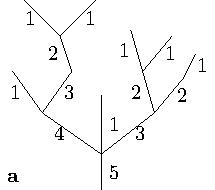
\includegraphics[width=4cm]{fig/stream_order.pdf}
        \DIFaddFL{\hspace{0.5cm}
        }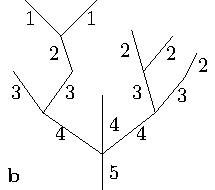
\includegraphics[width=4cm]{fig/stream_order_r.pdf}
        \DIFaddFL{\hspace{0.5cm}
        }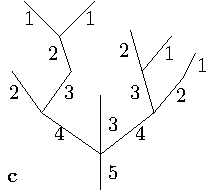
\includegraphics[width=4cm]{fig/stream_order_a.pdf}

        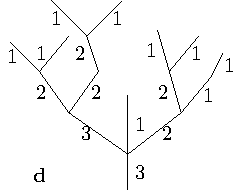
\includegraphics[width=4cm]{fig/stream_order_strahler.pdf}
        \DIFaddFL{\hspace{0.5cm}
        }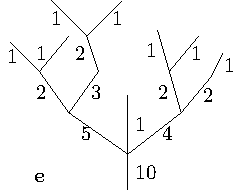
\includegraphics[width=4cm]{fig/stream_order_shreve.pdf}
    \end{center}
    \caption{\DIFaddFL{Illustration of and comparison between different stream ordering methods. }\textbf{\DIFaddFL{a}} \DIFaddFL{Lower limits of the feasible stream order values from our proposed mehods. }\textbf{\DIFaddFL{b}} \DIFaddFL{The upper limits of the feasible stream order values from our proposed methods. }\textbf{\DIFaddFL{c}} \DIFaddFL{Another feasible set of stream order values conforming the two rules of our proposed ordering methods as described in }\Cref{tab:zheng_order}\DIFaddFL{. }\textbf{\DIFaddFL{d}} \DIFaddFL{The Strahler stream ordering method. }\textbf{\DIFaddFL{e}} \DIFaddFL{The Shreve stream ordering method. }\label{fig:zheng_order}}
\end{figure}

\subsection{\DIFadd{Comparison with Existing Stream Ordering Methods}}
\label{sec:comparison}

\DIFadd{Our ordering method }\DIFaddend is inspired by several foundational studies. The mizuRoute river network routing model, for instance, employs the Strahler stream order to segment mainstreams into branches~\cite{mizukami2021JAMES}. Within each branches, reaches are sequentially simulated from upstream to downstream, while branches of the same Strahler order are processed in parallel. This approach underscores the potential of order-based parallelism. However, the Strahler \DIFdelbegin \DIFdel{order }\DIFdelend \DIFaddbegin \DIFadd{ordering method, as depicted in }\Cref{fig:zheng_order}\DIFadd{d, }\DIFaddend categorizes branches rather than individual reaches, \DIFdelbegin \DIFdel{which results in }\DIFdelend \DIFaddbegin \DIFadd{leading to }\DIFaddend a granularity too coarse for efficient parallel routing. The disparity in the number of branches across Strahler orders and in the number of reaches in a branch introduces significant variability in the computational load, posing a considerable challenge for load balancing and scalable parallel processing.

\DIFdelbegin %DIFDELCMD < \begin{figure}[H]
%DIFDELCMD <     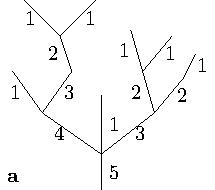
\includegraphics[width=4cm]{fig/stream_order.pdf}
%DIFDELCMD <     %%%
\DIFdelFL{\hspace{0.5cm}
}%DIFDELCMD < 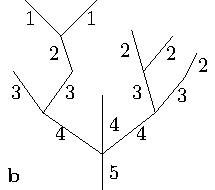
\includegraphics[width=4cm]{fig/stream_order_r.pdf}
%DIFDELCMD <     %%%
\DIFdelFL{\hspace{0.5cm}
}%DIFDELCMD < 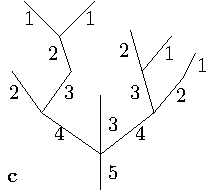
\includegraphics[width=4cm]{fig/stream_order_a.pdf}
%DIFDELCMD <     %%%
%DIFDELCMD < \caption{%
{%DIFAUXCMD
    \DIFdelFL{Illustration of the proposed stream orders. }\textbf{\DIFdelFL{a}} %DIFAUXCMD
    \DIFdelFL{The lower limits of the stream orders. }\textbf{\DIFdelFL{b}} %DIFAUXCMD
    \DIFdelFL{The upper limits of the stream orders. }\textbf{\DIFdelFL{c}} %DIFAUXCMD
    \DIFdelFL{A feasible set of stream order values conforming the two ordering rules. }%DIFDELCMD < \label{fig:zheng_order}%%%
}
%DIFAUXCMD
%DIFDELCMD < \end{figure}
%DIFDELCMD <

%DIFDELCMD < %%%
\DIFdel{In response to }\DIFdelend \DIFaddbegin \DIFadd{Recognizing }\DIFaddend these challenges, \DIFdelbegin \DIFdel{our proposed method }\DIFdelend \DIFaddbegin \DIFadd{a method that }\DIFaddend assigns stream orders directly to river reaches \DIFdelbegin \DIFdel{, enabling }\DIFdelend \DIFaddbegin \DIFadd{could enable }\DIFaddend more granular parallelization. The \DIFaddbegin \DIFadd{Shreve stream ordering method falls into this category. However, the method is too finely grained. The excessive granularity in the context of parallel routing can be demonstrated through the following theoretical reasoning: In an ideal scenario with unlimited processors, the computation time for parallel routing would be equivalent to that of computing the reaches sequentially along the longest flow path. For instance, as shown in Figure \ref{fig:zheng_order}e, there are five reaches along the longest flow path. An ideal ordering method would assign five unique order values, and the computation time would be five times the time required to compute a single reach. However, the Shreve method assigns six unique order values. If the number of processors is unlimited, the computation time would be six times the time taken to compute a single reach. This excessive granularity of the Shreve ordering leads to a suboptimal degree of parallelization.
}

\DIFadd{The }\DIFaddend Spatially Explicit Integrated Modeling System (SEIMS) model introduces a novel layer-based parallelism\DIFdelbegin \DIFdel{~}\DIFdelend \cite{liu2014EMS, liu2016EMS, zhu2019EMS}, \DIFdelbegin \DIFdel{where reaches are stratified }\DIFdelend \DIFaddbegin \DIFadd{which is considered to have an ideal granularity. The model stratifies reaches }\DIFaddend by their topological distance from the outlet. Reaches within the same layer are processed in parallel, with \DIFdelbegin \DIFdel{layers }\DIFdelend \DIFaddbegin \DIFadd{the layers being }\DIFaddend sequenced. Yet, the allocation of a reach to a specific layer is predetermined by the river network's topography. If the number of reaches in a layer does not \DIFdelbegin \DIFdel{align with }\DIFdelend \DIFaddbegin \DIFadd{match }\DIFaddend the number of processors, processor idleness ensues~\cite{liu2014EMS, zhu2019EMS}. \DIFdelbegin \DIFdel{The }\DIFdelend \DIFaddbegin \DIFadd{However, the }\DIFaddend SEIMS model lacks the flexibility required to optimize reach distribution across layers.

Our proposed \DIFdelbegin \DIFdel{stream }\DIFdelend ordering method offers a more adaptable alternative to the SEIMS model. \DIFdelbegin \DIFdel{The ordering is defined by two rules: (1) a reach's order falls within an integer range that is one more than the highest order of its upstream reaches and one less than the order of its downstream reach, and (2) the order value is an integer range from one up to the number of the reaches along the longest flow path within all the river networks under examination. This ordering ensures that reaches with identical orders are free from }\DIFdelend \DIFaddbegin \DIFadd{On one hand, the lower~(}\Cref{fig:zheng_order}\DIFadd{a) and upper~(}\Cref{fig:zheng_order}\DIFadd{b) bounds of our proposed orders parallel the SEIMS layers assigned using an }\DIFaddend upstream-downstream\DIFdelbegin \DIFdel{dependencies, allowing for parallel processing. }%DIFDELCMD <

%DIFDELCMD < %%%
\DIFdel{The ordering rules generate a spectrum of feasible }\DIFdelend \DIFaddbegin \DIFadd{~\mbox{%DIFAUXCMD
        \cite[Fig. 6b]{zhu2019EMS} }\hskip0pt%DIFAUXCMD
    and downstream-upstream~\mbox{%DIFAUXCMD
        \cite[Fig. 6c]{zhu2019EMS} }\hskip0pt%DIFAUXCMD
    strategy, respectively. Additionally, our proposed ordering method allows for variations in the }\DIFaddend stream order values \DIFdelbegin \DIFdel{. The }\DIFdelend \DIFaddbegin \DIFadd{between the }\DIFaddend lower and upper bounds\DIFdelbegin \DIFdel{of the feasible values for each reach can be estimated as follows, as shown in Figure~\ref{fig:zheng_order}. The lower bounds are calculated by repeating the following two steps: (1) assigning the upmost reaches an order of one, and (2) setting a reach's order to one plus the highest upstream order. This calculation parallels the upstream-downstream strategy utilized in SEIMS~\mbox{%DIFAUXCMD
        \cite[Fig. 6b]{zhu2019EMS}}\hskip0pt%DIFAUXCMD
    . Conversely, the upper bounds are determined by: (1) designating the outlet reach an order equivalent to the number of reaches along the longest flow path, and (2) subtracting one from the downstream reach 's order. This calculation aligns with the downstream-upstream strategy in SEIMS~\mbox{%DIFAUXCMD
        \cite[Fig. 6c]{zhu2019EMS}}\hskip0pt%DIFAUXCMD
    . The flexibility in stream order assignment provides an opportunity to optimize reach }\DIFdelend \DIFaddbegin \DIFadd{, provided that the two rules are satisfied. This flexibility enables the optimization of reach }\DIFaddend distribution, potentially minimizing processor idleness and enhancing parallel efficiency, as evidenced \DIFdelbegin \DIFdel{by our results}\DIFdelend \DIFaddbegin \DIFadd{in Section~\ref{sec:optimization_yangtze}}\DIFaddend .

\DIFdelbegin \DIFdel{As the }\DIFdelend \DIFaddbegin \DIFadd{Our proposed ordering method can also incorporate the halo-reach method to further enhance parallel scalability. If the }\DIFaddend number of processors \DIFdelbegin \DIFdel{increases significantly, }\DIFdelend \DIFaddbegin \DIFadd{allocated for parallel river network routing is sufficiently large, the }\DIFaddend computation time will predominantly be dictated by the reaches along the longest flow path. \DIFdelbegin \DIFdel{To further enhance parallel scalability, our proposed ordering methods can be complemented with halo reaches. }\DIFdelend By strategically inserting halo reaches upstream of select reaches along the longest flow path, the river network \DIFdelbegin \DIFdel{is }\DIFdelend \DIFaddbegin \DIFadd{can be }\DIFaddend effectively partitioned into subnetworks with shorter longest flow paths. \DIFdelbegin \DIFdel{The orders for these subnetworks and halo reaches are assigned according to the above proposed methods. The }\DIFdelend \DIFaddbegin \DIFadd{This partitioning will enable the application of our proposed ordering methods to each subnetwork, thereby enhancing parallel scalability. In comparison with the existing halo-reach method, the }\DIFaddend use of halo reaches \DIFaddbegin \DIFadd{with our proposed ordering method }\DIFaddend should be judicious, reserved for scenarios where the longest flow path emerges as the primary determinant of computation time. \DIFaddbegin \DIFadd{The judicious use will minimize the impact of inexact inflows to the artificially partitioned subnetworks, ensuring simulation accuracy.
}\DIFaddend

\subsection{A Conceptual Shared-Memory Parallel Execution Machine for River Network Routing}
\label{sec:parallel_machine}

In this study, we utilize a conceptual shared-memory parallel execution model to assess the parallel performance and scalability of our proposed stream ordering method. This model offers a theoretical framework for evaluation, factoring out the impact of inefficient code implementation and hardware architectural differences. The parallel performance and scalability metrics obtained are instrumental in guiding the optimization of the proposed stream orders.

The conceptual machine is equipped with $m$ processors capable of simultaneously processing up to $m$ reaches. The river networks under consideration comprise a total of $n$ reaches. The machine selects groups of reaches from the river networks, beginning with the lowest order. Each group consists of reaches of the same order, which are selected randomly. The size of each group not exceeding $m$. This process is repeated until all reaches have been simulated, as outlined in Algorithm~\ref{alg:shared_memory}.

We disregard the time spent on fetching and potential data saving operations. The total computation time is quantified by the total number of groups required to process the entire river network. Parallel performance is gauged using the metrics of parallel speedup and efficiency. Parallel speedup is calculated as the ratio of the computation time for sequential simulation (i.e., the total number of river reaches) to that for parallel simulation. Perfect scaling is achieved if the speedup ratio increases linearly with the number of processors. Parallel efficiency is determined by the ratio of actual parallel speedup to the ideal speedup under perfect scaling conditions. This efficiency metric is crucial for evaluating the parallel performance and scalability of the proposed stream orders.

During computation, there may be instances of processor idleness. This idleness is attributed to the mismatch between the number of reaches in a group and the number of available processors. Such idleness can diminish parallel efficiency and scalability. To identify potential sources of this idleness, we will calculate the computation deficiency for each individual reach. The computation deficiency of a reach is defined as the ratio of the number of idle processors during the routing of the reach to the number of total processors. If no processors are idle during the routing of a reach, the computation deficiency is zero. If idle processors are present, the computation deficiency is positive; as the number of idle processors increases, the deficiency approaches one. This metric is valuable for identifying reaches that contribute to processor idleness and for guiding the optimization of stream orders.

\begin{algorithm}
    \caption{A shared-memory parallel execution machine of river network routing.}
    \label{alg:shared_memory}
    \begin{algorithmic}
        \REQUIRE There are $n$ streams. $O_i \in \mathbb{Z}^{+}$ is the order of the $i$-th stream, $i = 1\cdots{}n$. The order is sorted: $O_{i+1} - O_i \ge 0$.
        \REQUIRE The machine has $m$ processors. $m \in \mathbb{Z}^{+}$.
        \ENSURE The simulation of a stream must be after its upstream.
        \STATE $i \gets 1$ \COMMENT{the first stream of a group}
        \STATE $j \gets 1$ \COMMENT{the last stream of a group}
        \WHILE{$i \le n$}
        \FOR {$k = 1$ \TO $m$}
        \IF {$i + k - 1 \le n$ \AND $O_{i + k - 1} = O_i$}
        \STATE $j \gets i + k - 1$
        \ENDIF
        \ENDFOR
        \STATE \textbf{Parallel Simulation} Simulate the streams from $i$ to $j$ in parallel.
        \STATE $i \gets j + 1$
        \ENDWHILE
    \end{algorithmic}
\end{algorithm}

\section{\DIFdelbegin \DIFdel{Study Domain and Data}\DIFdelend \DIFaddbegin \DIFadd{Experimental Design}\DIFaddend }
\label{sec:domain}

We applied the proposed stream ordering and order-based parallel routing methods to the Yangtze River, the largest river network in China. The river network is characterized by full connectivity among its reaches. This case provides a rigorous evaluation of out proposed methods at a substantial scale and under challenging conditions for parallel routing.

For the delineation of the Yangtze River network, we employed the Multi-Error-Removed Improved-Terrain Hydrography (MERIT-Hydro) dataset~\cite{yamazaki2017GRL, yamazaki2019WRR}, a global hydrography dataset with a 3 arc-second spatial resolution. This dataset includes a hydrologically adjusted digital elevation model, an eight-direction flow model, flow accumulation area, river channel width, and height above the nearest drainage. Our delineation process utilized the flow accumulation area and the eight-direction flow model. The threshold for the flow accumulation area was set at 20 km\textsuperscript{2} for catchment delineation and 10 km\textsuperscript{2} for river centerline extraction. The extraction yielded a single river network comprising 53,600 reaches \DIFdelbegin \DIFdel{.
}\DIFdelend \DIFaddbegin \DIFadd{(tributaries), which are shown in }\Cref{fig:domain}\DIFadd{. We utilized the connectivity of the extracted river centerlines for subsequent analyses and employed the river geometry for graphical illustrations. The instructions for accessing the data are detailed in the supplementary materials.
}\DIFaddend

\DIFaddbegin \begin{figure}[H]
    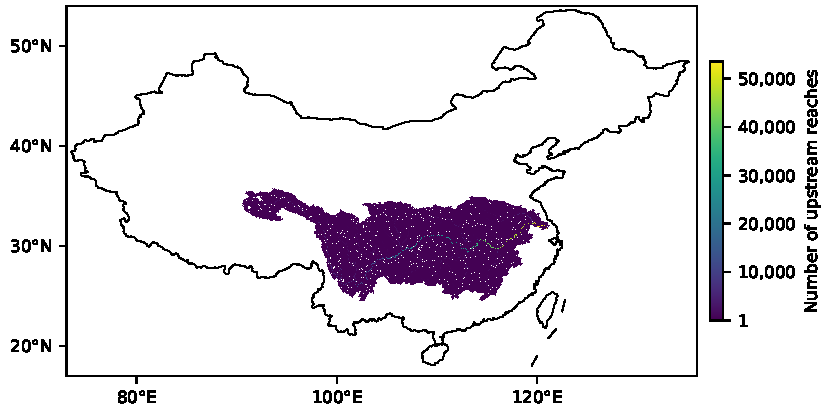
\includegraphics[width=14 cm]{fig/domain.pdf}
    \caption{\DIFaddFL{Yangtze River Basin Network delineated from the MERIT-Hydro dataset. The black lines outline the national boundaries or coastal lines of China, providing a geographical context. The color-coded lines depict the river reaches. Each color indicates the total number of reaches, encompassing the current reach and all upstream reaches }\label{fig:domain}}
\end{figure}

\DIFadd{Figure~\ref{fig:workflow} shows the workflow of this study. Initially, in Section~\ref{sec:stream_order_yangtze}, we assigned the Strahler, Shreve, and the upper and lower bounds of our proposed stream orders to the Yangtze River network, adhering to the rules detailed in Table~\ref{tab:zheng_order} and depicted in Figure~\ref{fig:zheng_order}. Subsequently, in Section~\ref{sec:parallelization_yangtze}, we assessed the computational performance of the Shreve order and the proposed stream orders' upper and lower bounds using a conceptual shared-memory parallel execution machine described in Section~\ref{sec:parallel_machine}. We measured this performance in terms of parallel speedup and efficiency and evaluated its scalability with an increasing number of processors. We also pinpointed hotspots of computational deficiencies. Lastly, in Sections~\ref{sec:optimization_yangtze} and \ref{sec:breakdown_yangtze}, we demonstrated that our proposed stream ordering method can be optimized, guided by the measured computation deficiencies, and can incorporate halo reaches into the longest flow path. This incorporation can significantly enhance computational performance and parallel scalability.
}

\begin{figure}[H]
    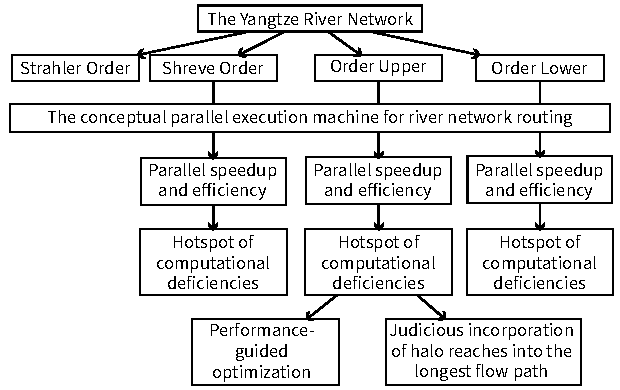
\includegraphics[width=10.5 cm]{fig/workflow.pdf}
    \caption{\DIFaddFL{Diagram of workflow }\label{fig:workflow}}
\end{figure}

\DIFaddend \section{Results \DIFaddbegin \DIFadd{and Discussion}\DIFaddend }
\label{sec:results}

\subsection{Stream Orders for the Yangtze River Network}
\label{sec:stream_order_yangtze}

\Cref{fig:spatial_distribution_yangtze} illustrates the spatial distribution of the proposed stream orders in the Yangtze River basin, juxtaposed with those of the Strahler and Shreve stream orders. The Strahler system exhibits a narrow range of order values, with a maximum value of eight observed in this case. This limited range restricts its application to parallelizing branches, akin to the mizuRoute model~\cite{mizukami2021JAMES}, rather than individual reaches. The coarse granularity of the Strahler order poses challenges for achieving effective load balancing.

In contrast, both the Shreve order and our proposed stream order offer \DIFdelbegin \DIFdel{adequate }\DIFdelend \DIFaddbegin \DIFadd{sufficient }\DIFaddend granularity for order-based parallel routing. It is important to note that the Shreve order is applicable for parallel routing only when no upstream-downstream pairs share the same order value, a condition that is coincidentally met in this study. However, the Shreve order spans a range from 1 to 26,828, which is excessively broad. As depicted in \Cref{fig:cumulative_count_yangtze}, 2,378 unique Shreve order values are assigned to only one reach. This \DIFaddbegin \DIFadd{indicates an excessive granularity that undermines the scalability of the parallel routing. No matter how many processors are allocated, only one can work at a time while the others remain idle, waiting for the routing on the reach to be completed. This }\DIFaddend extensive range, coupled with the scarcity of reaches sharing the same order value, can lead to inefficiencies in parallelization.

\Cref{fig:spatial_distribution_yangtze}c and \Cref{fig:spatial_distribution_yangtze}d display the spatial distribution of the lower and upper bounds of our proposed order family, respectively. These bounds range from 1 to 1,042, which corresponds to the number of reaches along the longest flow path. The upper bound demonstrates an even distribution of order values throughout the river network, while the lower bound shows a greater concentration in the lower order values. For the upper bound, a limited number of order values are assigned to a small set of reaches, as shown in \Cref{fig:cumulative_count_yangtze}. The balanced distribution of order values, along with the adequate granularity and the presence of sufficient reaches sharing the same order value, render the upper bounds of our proposed stream order family particularly well-suited for parallel river network routing.

\begin{figure}[H]
    \includegraphics[width=10.5 cm]{fig/spatial_distribution_yangtze.pdf}
    \caption{Spatial distribution of stream orders over the Yangtze River basin. \textbf{a} The Strahler order. \textbf{b} The Shreve order. \textbf{c} The lower bounds of the proposed order family. \textbf{d} The upper bounds of the proposed order family. \label{fig:spatial_distribution_yangtze}}
\end{figure}

\begin{figure}[H]
    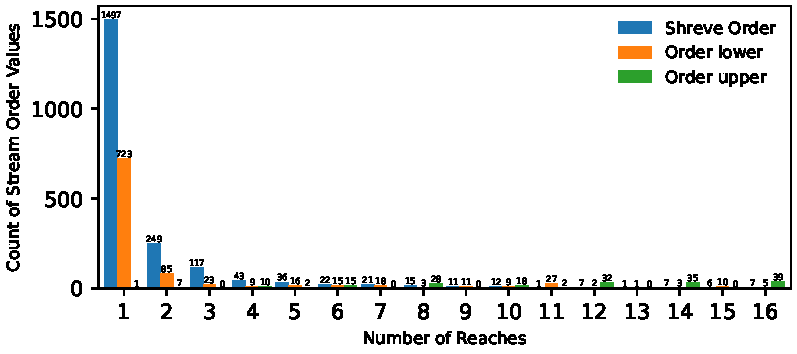
\includegraphics[width=13.5 cm]{fig/stream_count_yangtze.pdf}
    \caption{The count of stream order values with a limited number of reaches. For the sake of clarity, only those stream orders with 16 or fewer reaches are illustrated. \label{fig:cumulative_count_yangtze}}
\end{figure}

\subsection{Parallelization Performance, Scalability, and Hotspot of Computation Deficiencies}
\label{sec:parallelization_yangtze}

\Cref{fig:scalability_yangtze} displays the parallel speedup, efficiency, and scalability of the proposed stream orders compared to the Shreve order. Initially, as the number of processors increases, the ideal speedup is linearly proportional to the number of processors allocated. When the allocated processors become abundant enough, the parallelization process encounters a bottleneck due to the sequentiality along the longest flow path. The black dashed lines in the figure indicate this theoretical limit. In this instance, the number of processors at which the ideal speedup reaches the theoretical limit is 51, which corresponds to the ratio of the total number of reaches in the river network to the number of reaches along the longest flow path.

The Shreve order shows the lowest parallelization performance and scalability. Its efficiency falls below 80\% as soon as the processor count exceeds 6. When the number of processors is approximately 150 or above, the speedup is nearly saturated. The saturated speedup is significantly lower than the theoretical limit, with a value of approximately 24.5. This value is close to the ratio of the total number of reaches to the number of unique Shreve order values (i.e., 24.87). This indicates that the low saturated speedup is likely due to the broad range of Shreve order values and the scarcity of reaches sharing the same order value, as shown in \Cref{fig:spatial_distribution_yangtze} and \Cref{fig:cumulative_count_yangtze}.

The lower bounds of our proposed stream order family offer superior speedup and efficiency compared to the Shreve order. As the processor count increases, the parallel speedup increases more rapidly. Once the number of processors exceeds approximately 280, further increases have minimal impact on speedup. The saturation speedup closely matches the theoretical limit, indicating the granularity of our proposed stream order family is well-suited for parallel processing. The lower bounds also scale better. The efficiency remains above 80\% when the number of processors is less than 14.

The lower bounds of the proposed stream order family demonstrate better speedup and efficiency than the Shreve order. As the allocated processor count escalates, the parallel speedup increases at a more rapid rate than that of the Shreve order. However, once the number of processors surpasses about 280, the enhancement in parallel speedup becomes negligible. The saturation speedup is close to the theoretical limit, showing that the number of unique order values is appropriate. This suggests that our proposed stream order family is ideally granular for parallel river network routing. Additionally, the lower bounds showcase enhanced scalability, maintaining efficiency above 80\% when the processor count does not exceed 14.

The upper bounds demonstrated the best performance and scalability among the three methods. Efficiency is maintained above 80\% when the number of processors is 25 or fewer. As the number of processors increases, the speedup rapidly saturates, closely approaching the theoretical limits at a processor count of 141. These results indicate that the upper bounds of the proposed order family are particularly well-suited for parallel river network routing. The scalability of the upper bounds is either comparable to or surpasses those found in the existing literature~\cite{mizukami2021JAMES, liu2023JH}. It is important to note that scalability in this study is measured using a conceptual parallel execution model rather than with a real-world implementation.

\begin{figure}[H]
    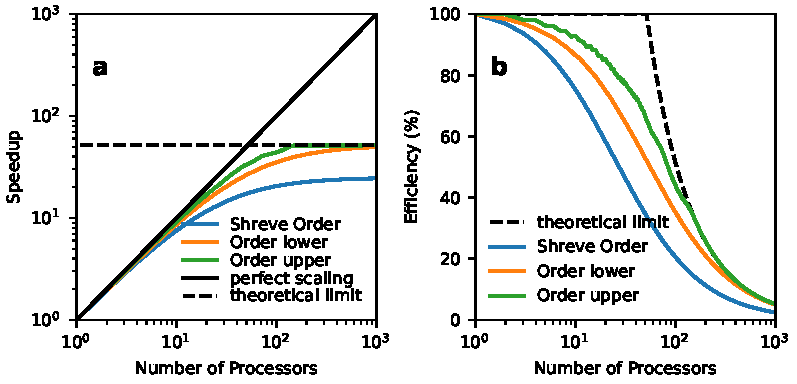
\includegraphics[width=13.5cm]{fig/speedup_yangtze.pdf}
    \caption{Parallelization speedup (\textbf{a}) and efficiency (\textbf{b}) for the Shreve orders and the proposed stream orders, respectively. The solid black lines represent the ideal speedup or efficiency under conditions of perfect scaling. The dashed black lines indicate the limits imposed by the upstream-to-downstream sequentiality along the longest flow path. \label{fig:scalability_yangtze}}
\end{figure}

\Cref{fig:computation_deficiency_yangtze} and \Cref{fig:computation_deficiency_hist_yangtze} respectively illustrate the spatial distribution and the histogram of computation deficiencies within the Yangtze River network. These deficiencies were measured using 51 processors, the point at which the ideal speedup aligns with the theoretical limit. For the Shreve order and the lower bounds of the proposed stream order family, reaches with significant computation deficiencies are primarily located in the mainstreams. This inefficiency arises from the limited number of mainstream reaches that share the same order values. In contrast, due to the coarse granularity of the upper bounds, the likelihood of computation deficiencies occurring is lower, and they are more concentrated.

The upper bounds exhibit a markedly different pattern, with reaches showing high computation deficiencies predominantly found in the upstream reaches, especially in the headwater regions. The greater number of upstream reaches, compared to mainstream reaches, makes it more probable that they will share order values. This sharing reduces the probability of processor idleness and computation deficiencies. The contrasting patterns observed between the lower and upper bounds suggest that there is considerable potential for optimizing the order values to improve parallel efficiency.

\begin{figure}[H]
    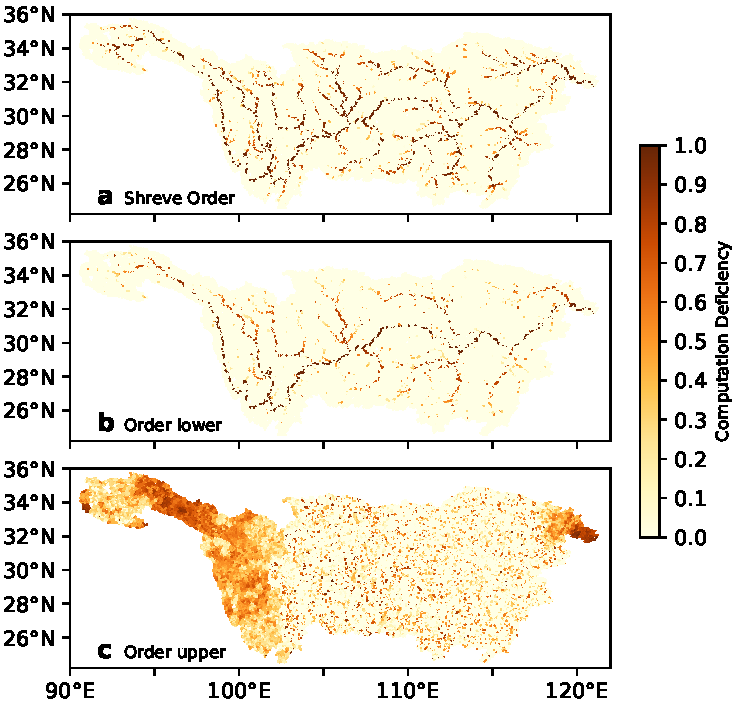
\includegraphics[width=11.5cm]{fig/computation_deficiency_yangtze.pdf}
    \caption{Computation deficiency of routing each individual reach observed at a processor count of 51 for the Yangtze River network. \label{fig:computation_deficiency_yangtze}}
\end{figure}

\begin{figure}[H]
    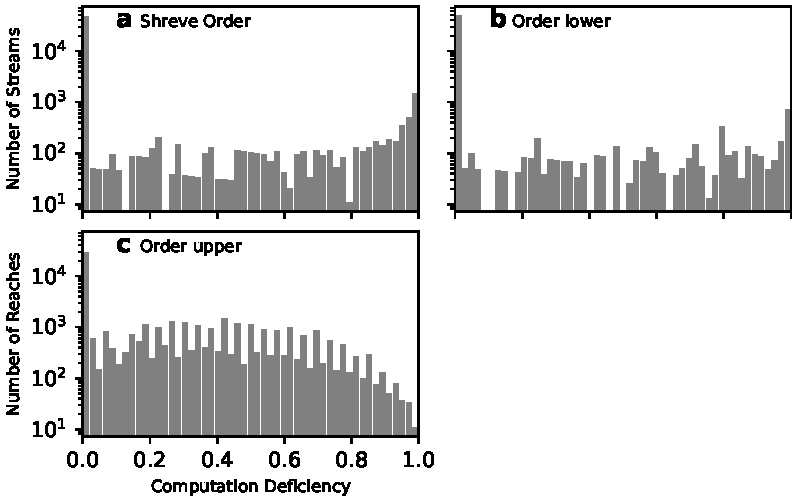
\includegraphics[width=13.5cm]{fig/computation_cost_hist_yangtze.pdf}
    \caption{Histogram of the computation deficiency for the Yangtze River network observed at a processor count of 51. \label{fig:computation_deficiency_hist_yangtze}}
\end{figure}

\subsection{\DIFaddbegin \DIFadd{Performance-Guided }\DIFaddend Optimization of the Stream Order in between the Two Bounds}
\label{sec:optimization_yangtze}

We show that the stream order can be optimized using a simple strategy that iteratively minimizes total computation time. The iterative optimization operates only on the reaches where the upper and lower bounds differ and starts with the upper bounds of the stream order family, which show the best parallel performance yet. In each iteration, the reach with the most significant computation deficiency is targeted, with its order being reduced by one. Concurrently, appropriate adjustments are made to the orders of upstream reaches to ensure adherence to the two rules outlined in \Cref{sec:stream_order}.

\Cref{fig:optimization_iteration_yangtze}a illustrates the reduction in total computation time at each optimization iteration. The total computation time experiences a rapid decline during the initial iterations, followed by a gradual stabilization. The stream orders that yield the minimum total computation time are then selected for further analysis. A comparison in the histograms of computation deficiencies between the optimized orders and the upper bounds of the stream order family is presented in \Cref{fig:optimization_iteration_yangtze}b. The optimization results in a slight reduction in the number of reaches with high computation deficiencies. \Cref{fig:optimization_iteration_yangtze}c displays the spatial distribution of computation deficiencies, showing that the optimization strategy effectively reduces these deficiencies, particularly in the middle reaches. However, the headwater and downstream regions exhibit negligible changes, indicating that a more advanced optimization strategy may be necessary to achieve enhanced parallel performance uniformly across the river network.

\begin{figure}[H]
    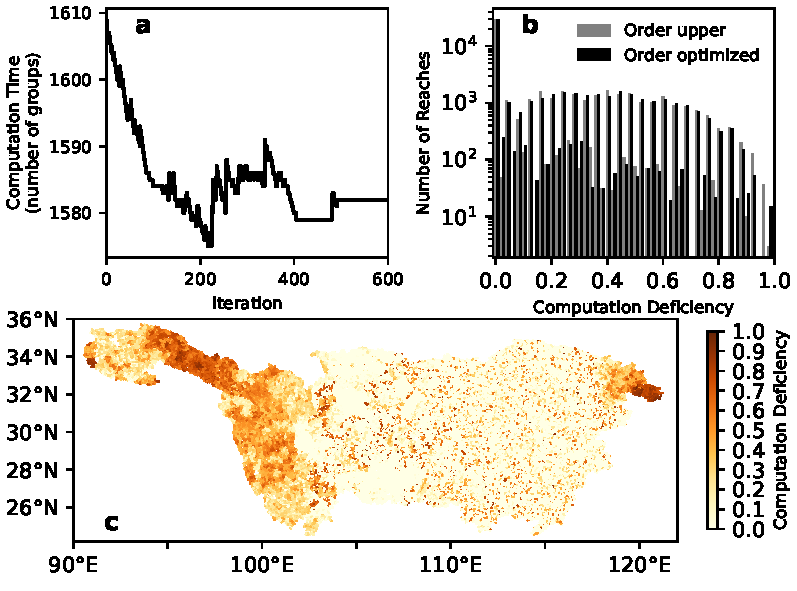
\includegraphics[width=13.5 cm]{fig/optimization_iteration_yangtze.pdf}
    \caption{Optimization of the stream order. \textbf{a} Decrease in the total computation time with the optimization iteration. \textbf{b} Comparison in the histogram of the computation deficiency for the optimized stream orders and the upper bounds of the stream order family. \textbf{c} Spatial distribution of the computation deficiency. \label{fig:optimization_iteration_yangtze}}
\end{figure}

\Cref{fig:order_optmization_yangtze} compares the upper bounds and the optimized stream orders for different number of processors. The optimized stream orders are obtained from iterations five times of the number of processors. The optimized stream orders exhibit a slight but consistent improvement in parallel speedup and efficiency, when the number of processors is limited. When the parallel performance of the upper bounds have already hit theoretical limits imposed by the sequentiality along the longest flow path, the optimized stream orders show no further improvement. These results suggest that relaxation of the upstream-to-downstream relationship is necessary for better parallel performance when the processor count is significant enough.

\begin{figure}[H]
    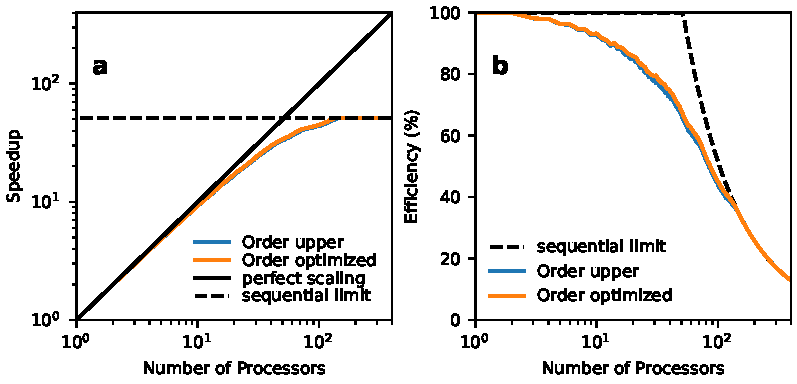
\includegraphics[width=12.5 cm]{fig/speedup_opt_yangtze.pdf}
    \caption{Same as \Cref{fig:scalability_yangtze} but for the optimized stream orders and the upper bounds of the proposed order family. \label{fig:order_optmization_yangtze}}
\end{figure}


\subsection{A few relaxations of the upstream-to-downstream relationship along the longest flow path}
\label{sec:breakdown_yangtze}

In this section, we introduce breakpoints along the longest flow path. The fully connected Yangtze river network is partitioned into independent subnetworks with these breakpoints. Halo reaches, which are duplicates of the upstream reaches at these breakpoints, are prepended upstream to the subnetworks. The inflow to the uppermost halo reaches is established and fixed during each routing time step and updated using the outflow from the upstream subnetworks before subsequent steps. We neglect the computation and communication time associated with these updates from our analysis, as our proposed parallel methods necessitate only a few breakpoints. In this study, we set the buffer length—--the minimum number of reaches along any flow path within the halo-reach region—--to six. The buffer length, approximately 80 km, is deemed sufficient to mitigate the impact of inexact inflows resulting from the relaxation~\cite{david2013WRR}. Apart from these adjustments, the segmented river networks can be processed using the ordering methods detailed in \Cref{sec:stream_order} and routed using the conceptual machine outlined in \Cref{sec:parallel_machine}.

\Cref{fig:spatial_distribution_breakdown_yangtze} illustrates the spatial distribution of the upper bounds of the stream orders for the Yangtze River network with one and three breakpoints. The breakpoints are placed in the equal intervals along the longest flow path. As analyzed above, the saturating parallel speedup equals to the ratio of the total number of reaches to the number of reaches along the longest flow path within the river networks. Such equally placed breakpoints can achieve the near-optimal saturating parallel speedup. However, the segmentation of the river network and appending of the halo reaches lead to the changes in part of the longest flow path. The placement of the breakpoints should be optimized by considering the interplay among the breakpoint insertion, halo reach appending, and the changes in the longest flow path. An optimization algorithm that can minimize the number of reaches along the longest flow path should be developed to achieve the best saturating parallel performance. However, such an optimization algorithm is beyond the scope of this study.

\Cref{fig:scalability_breakdown_yangtze} illustrates the parallel speedup and efficiency of the stream orders for the Yangtze River network with one and three breakpoints. As discussed, introducing breakpoints effectively raises the saturating parallel performance by shortening the longest flow path. The saturating parallel speedup can now exceed the theoretical limits imposed by the upstream-to-downstream sequentiality along the longest flow path. Moreover, the improvement in parallel speedup and efficiency is consistent across all different allocations of processor numbers. An 80\% parallel efficiency can be maintained for 40 processors with one breakpoint and for 77 processors with three breakpoints in the Yangtze River network. Performance saturation occurs when the number of processors exceeds approximately 150 and 280 for the network with one and three breakpoints, respectively. The enhancements in parallelization scalability are significant.

\begin{figure}[H]
    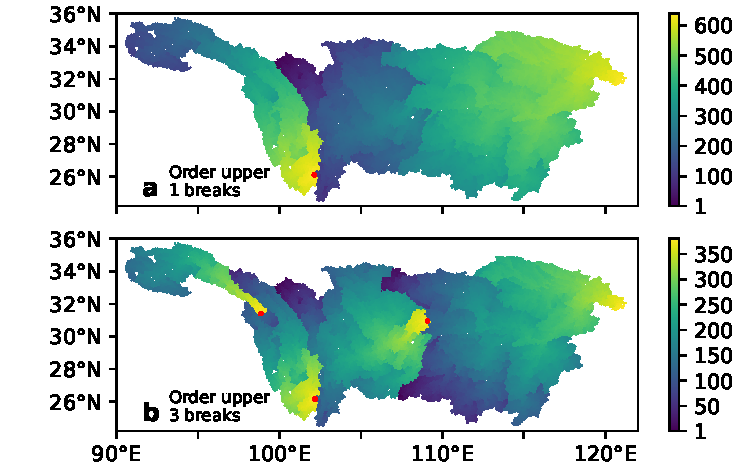
\includegraphics[width=10.5 cm]{fig/spatial_distribution_breakdown_yangtze.pdf}
    \caption{Same as \Cref{fig:spatial_distribution_yangtze}d, but for the stream orders with one (\textbf{a}) and three (\textbf{b}) breaks along the longest flow path. Red dots denote the breakpoints. The halo reaches are not shown for clarity. \label{fig:spatial_distribution_breakdown_yangtze}}
\end{figure}

\begin{figure}[H]
    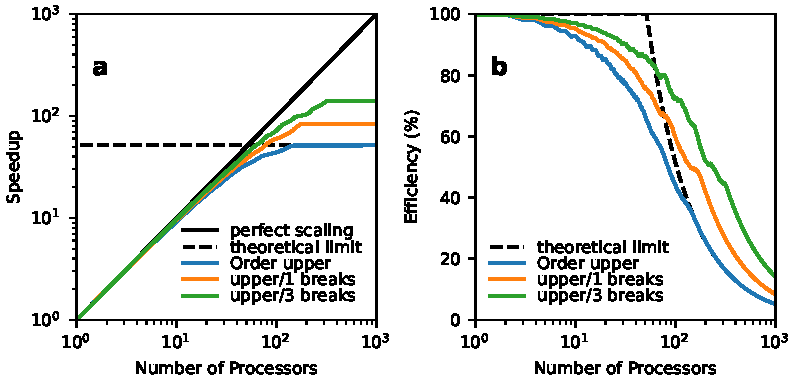
\includegraphics[width=13.5cm]{fig/speedup_bd_yangtze.pdf}
    \caption{Same as \Cref{fig:scalability_yangtze}, but for the upper bounds of the order family with two (the orange lines) or four (the blue lines) breaks along the longest flow path. \label{fig:scalability_breakdown_yangtze}}
\end{figure}


\section{\DIFdelbegin \DIFdel{Discussion and }\DIFdelend Conclusions}
\label{sec:conclusions}

In conclusion, this study introduces a novel family of stream orders and an associated order-based parallel routing method, designed to preserve the upstream-to-downstream flow sequence while facilitating parallel processing. The application of these methods within the Yangtze River basin has yielded superior performance and scalability, outperforming current strategies.

The potential for future research is abundant, with the optimization of stream orders and strategic placement of breakpoints offering promising avenues for further enhancing parallel performance. The findings of this study lay a solid theoretical groundwork for subsequent investigations in this domain.

\DIFdelbegin \DIFdel{Furthermore, the }\DIFdelend \DIFaddbegin \DIFadd{This study represents a pivotal step towards the development of more efficient modeling frameworks. The }\DIFaddend convergence of high-performance computing advancements \DIFdelbegin \DIFdel{and }\DIFdelend \DIFaddbegin \DIFadd{with }\DIFaddend the sophisticated numerical methods introduced \DIFdelbegin \DIFdel{herein }\DIFdelend \DIFaddbegin \DIFadd{in this research }\DIFaddend is poised to significantly \DIFdelbegin \DIFdel{advance land surface and Earth system modeling. By enabling the practical integration of }\DIFdelend \DIFaddbegin \DIFadd{enhance }\DIFaddend large-domain \DIFaddbegin \DIFadd{and }\DIFaddend fine-scale \DIFdelbegin \DIFdel{river network routing, forthcoming models}\DIFdelend \DIFaddbegin \DIFadd{flood forecasting capabilities. Future models, informed by our proposed methods, }\DIFaddend will be better \DIFdelbegin \DIFdel{positioned to simulate intricate hydrological processes}\DIFdelend \DIFaddbegin \DIFadd{equipped to capture the intricacies of river network dynamics}\DIFaddend , thereby enabling more precise and actionable \DIFdelbegin \DIFdel{forecasts. This research represents a pivotal step towards the development of more accurate and efficient modeling frameworks.
}\DIFdelend \DIFaddbegin \DIFadd{flood forecasts.
}\DIFaddend

\vspace{6pt}

% %% supplementary
%DIF < \supplementary{The following supporting information can be downloaded at:  \linksupplementary{s1}, Figure S1: title; Table S1: title; Video S1: title.}
\DIFdelbegin %DIFDELCMD <

%DIFDELCMD < %%%
\DIFdelend \authorcontributions{Conceptualization: H.Z.; methodology: H.Z.; software: H.Z.; validation: C.W. and Z.L.; formal analysis: X.Y.; investigation: X.Y.; resources: H.Y.; data curation: H.Z.; writing---original draft preparation: X.Y.; writing---review and editing: C.W. and Z.L.; visualization: X.Y. and H.Y.; supervision: H.Z.; project administration: H.Y.; funding acquisition: H.Y. All authors have read and agreed to the published version of the manuscript.}

\funding{This research was funded by the National Natural Science Foundation of China (grant number 42275178 and 42075165).}

\dataavailability{The MERIT hydrography dataset is available at \url{http://hydro.iis.u-tokyo.ac.jp/~yamadai/MERIT_Hydro} (accessed on 2024-05-01). The delineated river network, along with the scripts for river network analysis and figure generation used throughout this paper, can be found at the GitHub repository \url{https://github.com/hzheng88/paper-2024-stream-order-parallel-yangtze}.}

\conflictsofinterest{The authors declare no conflicts of interest.}

\begin{adjustwidth}{-\extralength}{0cm}
    %\printendnotes[custom] % Un-comment to print a list of endnotes

    \reftitle{References}

    \bibliography{references.bib}

    \PublishersNote{}
\end{adjustwidth}
\end{document}
